
\chapter*{Introduction}
\label{sec:org8d40cbd}
\section*{Motivation}
\label{sec:org00157a3}

\section*{Problem Statement}
\label{sec:orgbb18d2e}

\subsection*{Motivation}
\label{sec:org5d72463}
\emph{Can some device run a given algorithm?}

\emph{How the mapping process affect the circuit "probability of success"?}

\begin{figure}[htbp]
\centering
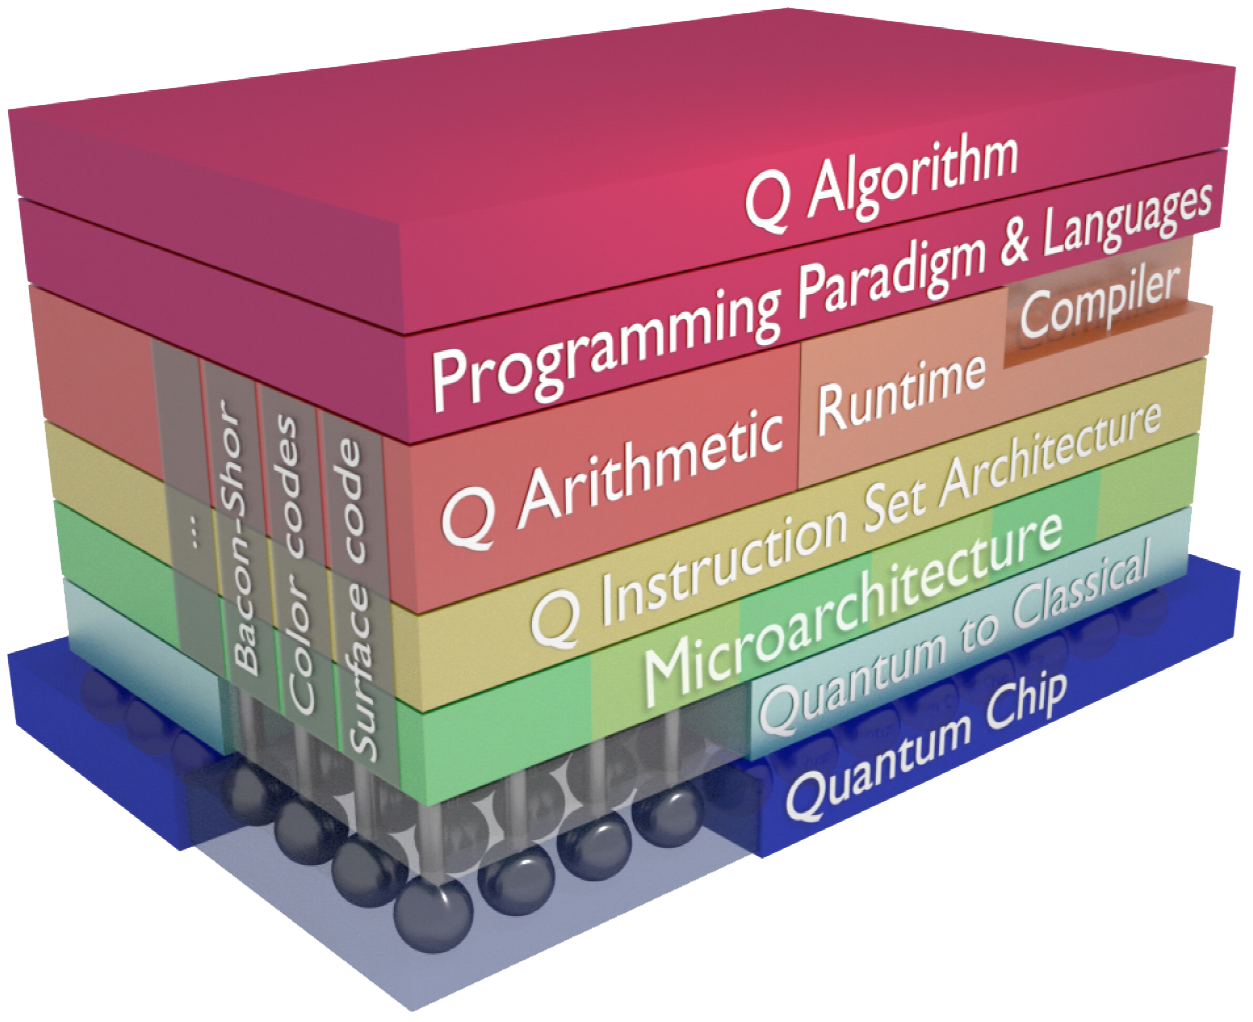
\includegraphics[width=0.7\textwidth]{figures/system_stack.png}
\caption{\label{fig:org0921a31}
Full stack implementation}
\end{figure}

\subsection*{Realization}
\label{sec:org1599963}
The work is centered in:

\begin{itemize}
\item SC-7 and SC-17 chips
\item Physical level, without error correction
\item Two error models:
\begin{itemize}
\item Pauli Noise (QX simulator)
\item Complex empirical error model (quantumsim)
\end{itemize}
\end{itemize}

\section*{Structure of the thesis}
\label{sec:org41c5786}
